\documentclass[10pt, a4paper, spanish]{article}
\usepackage[paper=a4paper, left=1.5cm, right=1.5cm, bottom=1.5cm, top=3.5cm]{geometry}
\usepackage[utf8]{inputenc}
\usepackage[spanish,es-nodecimaldot]{babel}
\usepackage{caratula}
\usepackage[pdfencoding=auto, colorlinks=true, linkcolor=blue]{hyperref}
\usepackage[boxruled, longend]{algorithm2e}
\usepackage{wrapfig}
% \usepackage{tikz}
\usepackage[rightcaption]{sidecap}
% \usetikzlibrary{babel}
\graphicspath{imagenes/}

% \tikzset{nodeList/.style={every node/.style={draw, circle}}}
% \tikzset{pathList/.style={every node/.style={midway, fill=white}}}


\newcommand{\ord}{\ensuremath{\operatorname{O}}}
\newcommand{\nat}{\ensuremath{\mathbb{N}}}

\begin{document}
% CARATULA
\materia{Sistemas operatornameerativos}
\submateria{Segundo Cuatrimestre de 2017}
\fecha{\today}
\grupo{}
\titulo{Trabajo Práctico 1}

\integrante{Tarrío, Ignacio}{363/15}{itarrio@dc.uba.ar}
\integrante{Szperling, Sebastián Ariel}{763/15}{sszperling@dc.uba.ar}
\integrante{Balbachan, Alexis}{994/12}{alexisbalbachan@gmail.com}

\maketitle

\newpage
\tableofcontents

\newpage
\section{Intro}
Además de la tabla de listas para cada entrada del mapa, decidimos agregar un contador de modificaciones, el cual tendrá dos utilidades en la clase, una es evitar que se ejecute addAndInc cuando se está ejecutando maximum y viceversa, y la otra es saber cuántas de estas se están ejecutando. Si el valor de este contador es positivo quiere decir que se están ejecutando ese número de addAndInc, y si es negativo se está ejecutando maximum. Para sincronizar correctamente los varios hilos de ejecución, utilizamos 2 mecanismos: por un lado, el contador está protegido por un mutex, para evitar que sea editado por 2 operaciones a la vez; y una variable de condición, que pone al thread en espera mientras la operación que desea realizar esté prohibida (por ejemplo, calcular maximum mientras se está agregando un elemento). También contamos con un arreglo de mutexes para bloquear cada lista individualmente mientras agregamos elementos.

\section{Ejercicio 1}
En el primer ejercicio se pide implementar el método push\_front de la lista atómica. Aquí tenemos crear un nuevo nodo y que este sea la nueva cabeza de la lista y que apunte a la vieja cabeza. El primer problema que nos cruzamos fue que primero realizabamos un exchange atómico de la cabeza antigua con el nuevo nodo y luego se lo apuntaba la la nueva cabeza. Este conjunto de operaciones no era atómico por lo que en ciertas situaciones si justo se intentaba de iterar la lista en el medio de estas dos operaciones habría una condición de carrera en la que la lista podría contener un solo elemento. Esto se solucionó aplicando la función atómica compare\_exchange\_weak a la vieja cabeza de la lista, asegurando que el nuevo nodo siempre apunte al último nodo agregado exitosamente.


\newpage
\section{Experimentación}

Hicimos unas pruebas del tiempo de ejecución de las dos versiones de

\begin{center}
	\texttt{static pair<string, uint> ConcurrentHashMap::maximum\\(uint p\_archivos, uint p\_maximos, list<string> archs);}
\end{center}

correspondientes a los ejercicios 5 y 6 del trabajo práctico. La versión del ejercicio 5 no utiliza la versión concurrente de \texttt{ConcurrentHashMap::count\_words}, y la versión del ejercicio 6 (llamada \texttt{maximum\_6} para desambiguar) sí.

\begin{center}
	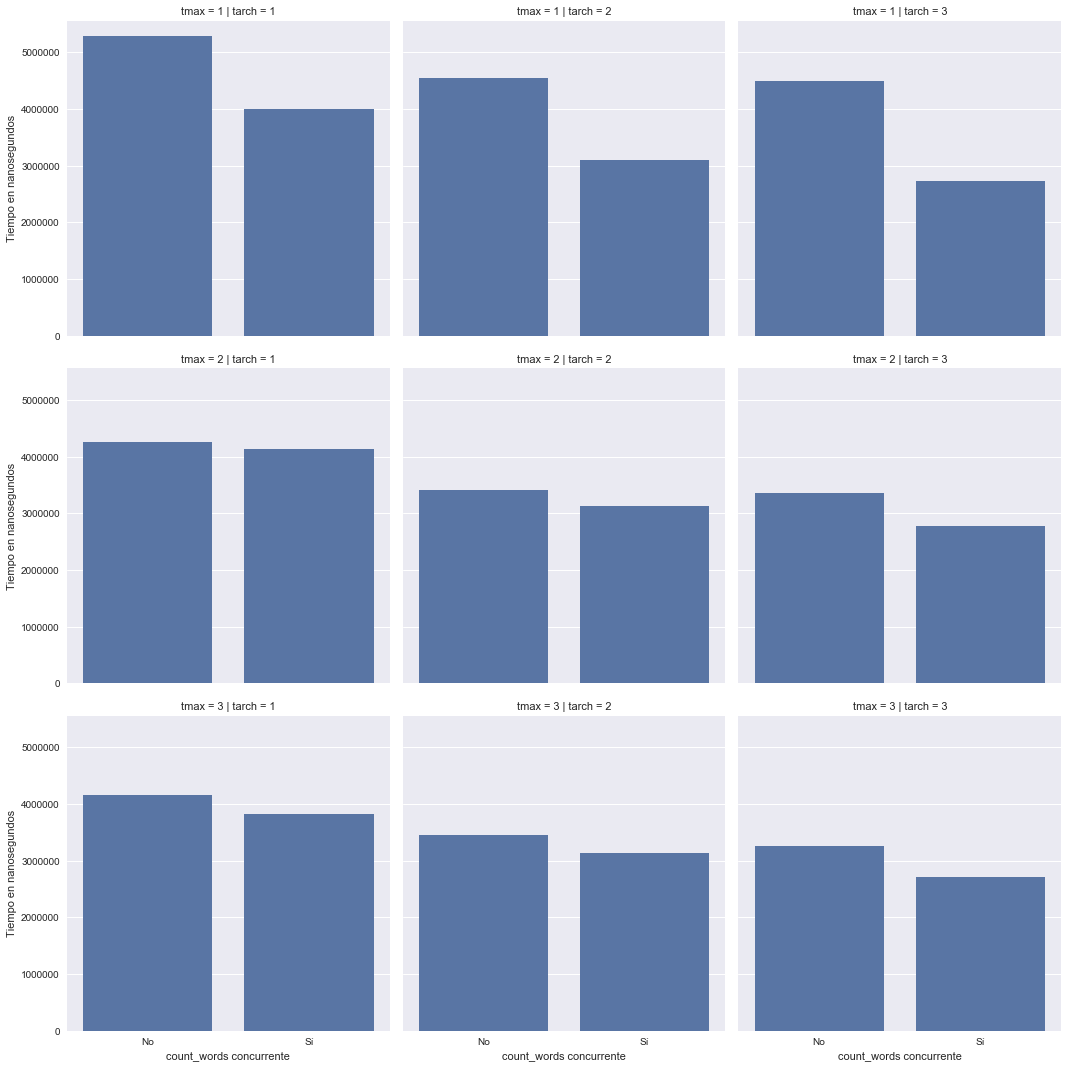
\includegraphics[scale=0.45]{imgs/5-vs-6.png}
\end{center}

En este gráfico se pueden apreciar 2 cosas:

\begin{itemize}

	\item la mejora de performance al utilizar threads es muy notoria, aunque la diferencia al agregar el 2do thread es mayor a la de agregar el 3er thread;

	\item la función que utiliza la versión con concurrencia de \texttt{ConcurrentHashMap::count\_words} puede hacer mejor uso de los threads que tiene disponibles, en particular durante la carga de los archivos, lo que era esperable ya que en la versión no concurrente se generan varios HashMaps y se deben copiar esos resultados a un único HashMap. También suponemos que, dado que todos los HashMaps almacenan sus datos en orden y tienen mutexes por fila de la tabla, es posible que haya muchas esperas durante la copia al HashMap unificado.

\end{itemize}

% compilar 2 veces para actualizar las referencias


\end{document}